\subsubsection{Liouville 理论的类比}\label{analiouville}

尽管本文并不需要这一事实，我们仍应指出：Virasoro 共形块与 Chern-Simons 理论之间的关系，可以简单地推广为 Liouville 理论与 Chern-Simons 理论之间的关系。为在黎曼面 $C$ 上研究 Liouville 理论，人们考虑 $C\times I$ 上的 Chern-Simons 理论，其中 $I$ 是单位区间。在 $I$ 的一端施加 Nahm 极点边界条件，在另一端则施加一个把 $z$ 与 $\bar z$ 互换的 Nahm 极点边界条件变体。Liouville 配分函数与关联函数由全纯和反全纯 Virasoro 共形块组合而成，而这些共形块自然地来自带有上述边界条件的 $C\times I$ 上的 Chern-Simons 理论。（对于紧致对称群的情形，人们已经知道 $C\times I$ 上的 Chern-Simons 理论能够重现 $C$ 上的 WZW 模型。）把我们眼下即将给出的论证稍加推广即可看出：插入在点 $p\in C$ 处的 Liouville 理论的轻退化场与一般初级场，对应于 $p\times I$ 上的 Wilson 算符或单值性缺陷。

在经典极限下，Chern-Simons 理论与 Liouville 理论之间的对应意味着以下内容。带有上述边界条件的 $C\times I$ 上 Chern-Simons 理论的经典解，是 $C$ 上的一个平坦丛，其全纯结构与反全纯结构都满足 oper 条件。确实，Liouville 理论的经典解对应于 $C$ 上一个常负曲率的度规。若 $\omega$ 与 $e$ 分别是该度规的标架（vierbein）与自旋联络，那么我们就能定义相应的 $SL(2,\R)$ 平坦联络 $\A=\omega {\ct}_3+
e_{ z} \ct_++e_{\bar z}\ct_-$。取 $\ct_i$ 的标准表示，则 $\A_z$ 是上三角的，其右上角矩阵元处处非零；而 $\A_{\bar z}$ 是下三角的，其左下角矩阵元处处非零。因此，由该平坦联络定义的全纯结构与反全纯结构都满足 oper 条件，正如在 Chern-Simons 描述中所预期的那样。（反全纯 oper 结构的定义，是把“上三角”矩阵与“下三角”矩阵的角色互换。）于是，这就给出了两个理论在经典层面的映射。



\subsection{Wilson 线算符}\label{wilson}

为进一步理解从带 oper 边界条件的三维 Chern-Simons 理论到二维 Virasoro 共形块的映射，我们将探讨 Wilson 线算符在这一对应中的解释。首先回顾一下：若采用把 Chern-Simons 理论与流代数联系起来的标准边界条件，情形会如何。在此情形下，终止于三维流形 $M_3$ 边界上的 Wilson 线算符，代表在 WZW 共形块中于该边界点处插入一个共形初级场。若该 Wilson 线算符在 $G$ 的有限维表示 $R$ 中变换，则相应的共形初级场也在同一表示中变换。这与下述事实一致：终止于边界上的 Wilson 线算符不是规范不变的，而是在表示 $R$ 中变换，正如 WZW 模型中相应的初级场一样。

终止于施加 Nahm 极点边界条件的边界上的 Wilson 线算符，其类似的解释又是什么？Nahm 极点破坏了边界处的规范对称性，因此我们必须选取 Wilson 线算符的某个分量。正如我们在第~\ref{flatpole}~节中所讨论的，一般的矢量平行移动到边界时会发散。给定一个终止于 $y=0$ 的 Wilson 线算符，最容易定义的规范不变信息是 $y$ 的最负幂次的系数。只需与小截面 $s$ 的适当幂次缩并，即可提取出这个系数。事实上，我们会发现 $s$ 的一个重新标度版本很有用，即 $\hat s = K(z)^{-1/2} s(z)$，它满足
\begin{equation}
\left( \D_z^2 + t(z) \right) \hat s=0 \qquad \D_{\bar z} \hat s =0 \qquad \D_{y} \hat s = 0
\end{equation}
并且具有确定的共形维数 $-1/2$。在规范 (\ref{torog}) 下，$\hat s=\begin{pmatrix}0\cr 1\end{pmatrix}$。

% [Tutor Note: 易错点] 注意 $K(z)$ 不是度规分量，而是前文定义的 $K(z)=\prod_a(z-z_a)^{k_a}$（它编码奇异磁单极子的位置与荷，并满足 $p(z)Q(z)^2=K(z)$）。由 $s\wedge \D_z s=K(z)$ 可知 $s$ 的量级为 $K^{1/2}$，故乘以 $K(z)^{-1/2}$ 恰好把奇性抵消，使 $\hat s$ 正则且成为共形权 $-1/2$ 的对象，从而在规范 (\ref{torog}) 下可取 $\binom{0}{1}$。若漏掉这个重标度因子，后面"与 $\hat s^{\,k}$ 缩并给出维数 $-k/2$"的记账就不再成立。

在 $SU(2)$ 的二维表示中，我们会考虑算符
\begin{equation}\label{zello}
P \exp \left (-\int_\gamma \A\right)  \hat s(z),
\end{equation}
其中 $\gamma$ 是终止于 $y=0$ 边界上的路径。在经典极限下，在边界的共形变换下，该算符具有与 $\hat s$ 相同的共形维数，即 $-1/2$。对于自旋 $k/2$ 表示，必须与 $\hat s$ 的 $k$ 次幂缩并，此时维数的经典极限为 $-k/2$。

% [Tutor Note: 物理图像] Wilson 线本身只负责把表示 $R$ 从体内部“输运”到边界，真正的物理信息在于它如何与边界上那支被 Nahm 极点选出的方向缩并。可以把 $\hat s$ 理解为 Nahm 极点所定义的边界“真空方向”：缩并 $\hat s^{\,k}$ 就是在把自旋 $k/2$ 的算符投影到该方向上，这正是它对应 Liouville 轻退化场的几何来源。

我们现在要论证：带有终止于边界上的自旋 $k/2$ Wilson 算符的 Chern-Simons 路径积分，给出一个 Virasoro 共形块，其中插入了 Liouville 动量为 $-b k/2$ 的“轻”退化场。这样的场在 $b \to 0$ 极限下具有正确的经典维数 $-k/2$；而且其量子维数的精确公式
\begin{equation}
-\frac{k}{2} b\left(b+\frac{1}{b} + \frac{k}{2} b\right) = -\frac{k}{2} - \frac{k(k+2)}{4}b^2=-\frac{k}{2}
+\frac{k(k+2)}{4(\k+2)}
\end{equation}
等于 $\tilde s^k$ 的经典维数与 WZW 模型（能级为 $\k+2=-1/b^2$，如式 (\ref{bpar}) 所示）中自旋 $k/2$ 算符的维数之和。此外，算符 (\ref{zello}) 在经典层面满足正确的微分方程：$k=1$ 的算符被 $\partial_z^2 + t(z)$ 湮灭，依此类推。

% [Tutor Note: 易错点] 该式最后一个等号用到式 (\ref{bpar}) 的 $b^2=-1/(\k+2)$：把 $-\frac{k(k+2)}{4}b^2$ 中的 $b^2$ 换成 $-1/(\k+2)$ 即得 $+\frac{k(k+2)}{4(\k+2)}$，符号翻转是这一步的关键，切勿漏掉负号。另外注意此处的"量子维数"指退化场的总维数（经典部分加 WZW 部分），其 $b\to0$ 的领头项才是 $-k/2$。

% [Tutor Note: 省略证明] 作者称经典层面“满足正确的微分方程”，实际上只对 $k=1$ 给出了 $\partial_z^2+t(z)$ 的验证范例：$k=1$ 时 $\hat s$ 本身被该算符湮灭，一般 $k$ 的情形要由 $\hat s$ 的各次乘积在 $t(z)$ 的奇点附近的算符乘积展开逐项核对，原文省略了这一归纳步骤。

这其中有一部分原因在于：退化场所满足的融合规则，与 WZW 模型中自旋 $k/2$ 算符的融合规则相吻合，从而使自旋 $k/2$ Wilson 线与退化共形场之间的对应成为可能。后一事实正是下述陈述的部分依据：与 Jones 多项式相伴的辫群表示，既可以通过 WZW 模型初级场的编织来计算，也可以通过 Virasoro 代数退化共形场的编织来计算。

\subsection{奇异磁单极子与“重”退化场}\label{hdf}
接下来，我们想在 Virasoro 共形块的 Chern-Simons 描述中辨认出 Liouville 动量为 $-k/2b$ 的“重”退化场。这些退化场的共形维数在 $b\to 0$ 时发散。我们断言：它们对应于在边界处插入奇异磁单极子。

% [Tutor Note: 约定差异] 请留意“轻/重”的区分完全由 $b\to0$ 的标度决定：轻退化场的动量正比于 $b$，维数在 $b\to0$ 时保持有限（如上一小节的 $-k/2$）；重退化场的动量正比于 $1/b$，维数按 $1/b^2$ 发散。因此同一族退化场在 $b\to0$ 与 $b\to\infty$ 两种极限下的“轻/重”身份会互换，阅读后续文献时务必先确认其 $b$ 的极限方向。

第~\ref{opsing}~节的主要洞见是：在带有奇异磁单极子（且 $\zeta$ 取一般值）的 Nahm 边界处，联络是一个带平凡单值性奇点的 oper。我们观察到，此类 oper 的经典应力张量的极点，与存在重退化场时量子应力张量的半经典极限相吻合。此外，平凡单值性条件在量子层面同样成立：轻退化场绕重退化场没有单值性，因为它们在唯一的道中融合。

% [Tutor Note: 物理图像] “重退化场绕一圈无单值性”这句话应反过来读：之所以无单值性，是因为重场在融合规则中只允许唯一道，轻场绕它一圈后回到自身的同一分量，故 $\mathcal M$-矩阵为纯数 $1$。这与非退化的一般初级场形成对照——后者绕重场一圈会被单值性矩阵混合，这正是算符乘积展开中出现的单值性。

在 Chern-Simons 的框架下，经典的平凡单值性条件自然来自下述事实：奇异磁单极子并不向体内部延伸。这是我们第~\ref{opsing}~节推导的一部分。在量子层面，我们需要考虑当轻退化场——在三维中由形如 $P\exp\left(-\int_\gamma\A\right) \hat s$ 的表达式表示——趋近奇异磁单极子时的行为。Wilson 圈本身是拓扑的，而小截面 $\hat s$ 绕奇异磁单极子具有平凡单值性。

\subsection{将各部分拼合起来}\label{punchline}
现在，我们终于可以建立出发时的四维 BPS 方程 (\ref{bpseqns}) 的解，与和 Jones 多项式相伴的辫群表示之间的联系。

BPS 方程的不含时解对应于具有平凡单值性的 oper。我们已经把相应量子态的编织，先等同于 Chern-Simons 理论中复积分链的编织，再等同于退化 Virasoro 共形块的编织。文献~\cite{Lawrence,SV} 指出，这些正是与 Jones 多项式相伴的辫群表示。于是我们抵达了目标，尽管形式听起来可能稍显抽象。

利用共形块的自由场表示，我们可以把这一结果表述为完全具体的形式。具有平凡单值性的 oper 也与 Bethe 方程的 Yang-Yang 函数的临界点相关联；后者是共形块自由场实现中被积函数的对数。退化 Virasoro 共形块既可以由与具有平凡单值性的 oper 相伴的无穷维针（thimble）导出，也可以由与 Yang-Yang 函数临界点相伴的有限维针导出。无论采用哪种方式，我们都得到在 $b^2$ 平面中角宽度大于 $\pi$ 的扇区内具有确定且一致半经典极限的共形块。由于这样的共形块是唯一的，这两组共形块的基必须重合。

因此，与四维规范场论相伴的编织表示，等同于 Bethe 参数 $w_i$ 空间中积分链的编织表示。若开启一个对称性破缺参数，这一点就不像乍看之下那样令人惊讶：此时我们把 $w_i$ 解释为体内部 BPS 磁单极子的位置，而我们的断言或许无非是说，库仑分支上的四维非阿贝尔规范场论约化为一个由大质量磁单极子与阿贝尔规范场构成的理论。我们将在第~\ref{supermon}~节进一步发展这一观点。

\section{积分链的编织表示}\label{brrep}

\begin{keytakeaways}
\begin{itemize}\setlength{\itemsep}{2pt}
  \item \textbf{物理图像}：Virasoro 退化共形块可用自由场表示写成对中间维数积分链 $\Gamma$ 的积分，被积函数的指数为 Yang-Yang 函数 $\W/b^2$；$\W$ 的临界点即 Bethe 方程的根，对应体内部 BPS 磁单极子的位置。
  \item \textbf{数学工具}：Morse 理论给出积分链的一组标准基——与 $\W$ 各临界点相伴的针（thimble）；针基下的编织矩阵元是 $q$ 的整系数 Laurent 多项式，而在常规定义的 BPZ 闭合围道基下则不具备这种初等性。
  \item \textbf{主要结论}：与四维规范场论相伴的辫群表示，等同于 Bethe 参数空间中积分链的编织表示；在无对称性破缺时，非紧的针同调等价于 $w_i$ 绕 $z_a$ 的紧致围道。
  \item \textbf{约定要点}：$G=SU(2)$（$k_a$ 全偶）时 $\W$ 模 $2\pi i$ 良定义、编织矩阵为 $q$ 的 Laurent 多项式；$G=SO(3)$（可有奇数 $k_a$）时 $\W$ 仅模 $2\pi i/4$ 良定义，编织矩阵实为 $q^{1/4}$ 的 Laurent 多项式。
\end{itemize}
\end{keytakeaways}

\subsection{概述}\label{moreover}

我们迄今所学内容的一个亮点是：存在一个自然的映射，从由四维规范场论方程 (\ref{bpseqns}) 导出的辫群表示，映入与 Virasoro 退化场关联函数相伴的辫群表示。这些辫群表示可以利用自由场表示来有效地研究，而该表示我们已在第~\ref{opbl}~节回顾过。把这一点明确写出来，正是我们此处的目标。

我们考虑退化关联函数 $\left\langle \prod_{a=1}^d V_{-k_a/2b}(z_a)
\right\rangle$。假定 $z_a$ 是 $\C$ 中互不相同的点。为表示共形块，我们引入 $q$ 个变量 $w_i\in \C$，并假定它们彼此不同，也与 $z_a$ 不同。$q$ 的允许取值已在第~\ref{analog}~节中分析过。此外，我们把 $w_i$ 视为不可区分的，即彼此只差一个置换的构型是等价的。我们用 $\M$ 表示这种互不相同且不可区分的变量 $w_i\in \C\backslash\{z_1,\dots,z_d\}$ 构成的空间。同时记 $\hat \M$ 为 $\M$ 上使式 (\ref{yy}) 中的 Yang-Yang 函数 $\W$ 单值化的最小覆盖。

在自由场表示中，退化共形块写成如下形式
\begin{equation}\label{dolf}\int_\Gamma \exp\left(\W/b^2\right)\,\d w_1\dots
\d w_q.\end{equation} $\Gamma $ 是 $\hat\M$ 中的一个中间维数的链，其选取使积分收敛。\footnote{如文献~\cite{Lawrence} 所述，链 $\Gamma$ 实际上应当在任意一对 $w$ 交换时变号，以补偿微分形式 $\d w_1\wedge\dots\wedge\d w_q$ 在置换下发生的符号改变。这意味着，相应的相对同调实际上是关于 $w$ 的置换反对称的那一部分。具体地说，设有两个 $w$，并且我们找到 Bethe 方程的一个解，使 $w$ 在置换意义下分别等于 $\alpha$ 与 $\beta$。那么我们可以定义一个与临界点 $w_1=\alpha$、$w_2=\beta$ 相伴的链 $\CC'$，以及一个与临界点 $w_1=\beta$、$w_2=\alpha$ 相伴的链 $\CC''$。差 $\CC'-\CC''$ 是同调的反对称部分的一个元素。实际操作中，我们可以略去显式构造这类差，并且忽略由 $\d w_1\wedge\dots\wedge \d w_n$ 中各因子的置换所产生的负号。}

% [Tutor Note: 含糊点拨] 脚注中“链应在交换 $w$ 时变号”这一要求是技术性的：$\M$ 已经把 $w_i$ 当作不可区分的点，取其覆盖 $\hat\M$ 后置换会给出不同的叶；微分形式 $\d w_1\wedge\dots\wedge\d w_q$ 在置换下变号，若不同时要求链反对称，积分就不是置换不变的。实际计算中（如 \cite{Lawrence}）通常直接按全纯微分形式的规范固定来算，只在成对比较时记住这个符号。

Morse 理论提供了一种系统地产生所有这类积分链的方法：积分链的一组基由与 $\W$ 的临界点相伴的针给出。这类链从来不是紧致的；它们带有非紧的端点，在其上 Morse 函数 $h = \mathrm{Re} \,\W$ 趋于 $-\infty$。在我们的问题中，这发生在某个 $w_i$ 趋近于某个 $z_a$ 时，或者在存在对称性破缺时，它沿正确方向趋于无穷时。在简单情形下，可以不用 Morse 理论而手工描述积分链。手工构造链 $\Gamma$ 时，必须确保 Morse 函数沿 $\Gamma$ 在无穷远处确实趋于 $-\infty$。例如，若有太多 $w_i$ 同时趋近同一个 $z_a$，这一点就会失效。

在存在对称性破缺时，一些重要的积分链终止于 $w=\infty$，非紧积分链的使用不可避免。然而，在不存在对称性破缺时，Morse 理论产生的非紧积分链的端点位于 $w_i\to z_a$（对不同的 $i$ 与 $a$），并且在适当的扭化相对同调中，等价于 $w_i$ 以适当方式绕过 $z_a$ 的紧致链。（例子可参见下文图~\ref{compare}。）在关于共形块自由场实现中积分链的广泛文献~\cite{DF,Felder} 及其在 Jones 多项式中的应用的文献~\cite{Lawrence,SV} 中，人们常常使用紧致积分链。据我们所知，对称性破缺——换言之，在无穷远处引入非正则奇点——在这一语境下尚未被考虑过。

使用 Morse 理论有利也有弊。主要的缺点在于，针并不对应于由退化场在特定道中融合所定义的标准 BPZ 共形块基。主要的优点在于，在针基下，辫群明显地由矩阵表示，而这些矩阵的矩阵元是 $q$ 的整系数 Laurent 多项式。这一性质（已在第~\ref{nonsingle}~节说明）对于 Jones 多项式与 Khovanov 同调而言十分重要。

在下文中，我们将首先分析几个重要例子，其中退化插入 $z_a$ 与 Bethe 根 $w_i$ 的数目都很少，无论有无对称性破缺。然后在第~\ref{genpicture}~节中，我们分析存在对称性破缺的一般情形。由这一分析，我们将获得推导 Jones 多项式的一般描述（而不只是相伴的辫群表示）所需的经验。相关内容在第~\ref{abdesc}~节给出。

\subsubsection{$SU(2)$ 与 $SO(3)$ 的对比}\label{contrast}

我们在此稍作停顿，就“编织矩阵的矩阵元是 $q$ 的 Laurent 多项式”这一论断作一点技术性说明。

若规范群为 $G=SU(2)$，即对偶群为 $G^\vee=SO(3)$，且奇异磁单极子的荷 $k_a$ 全为偶数，则 (\ref{yy}) 所定义的 Yang-Yang 函数 $\W$ 在模 $2\pi i$ 意义下良定义。于是 $\W$ 的分支改变会使 $\exp(\W/b^2)$ 乘以 $q=\exp(-2\pi i/b^2)$ 的整数次幂，从而编织矩阵是 $q$ 的整系数 Laurent 多项式。

反之，若 $G=SO(3)$、$G^\vee=SU(2)$，则某些 $k_a$ 可以为奇数。（事实上，我们的详细计算将针对所有 $k_a$ 均为 1 的情形。）此时，若纽结位置 $z_a$ 固定而改变 $w_i$，$\W$ 在模 $2\pi i$ 意义下良定义；但当 $z_a$ 变动时，它只在模 $2\pi i/4$ 意义下良定义。因此，对 $G=SO(3)$，编织矩阵实际上是 $q^{1/4}$ 的 Laurent 多项式。

% [Tutor Note: 易错点] 这里 $q^{1/4}$ 的出现不是笔误，而是 $SO(3)$ 规范场论中 Chern-Simons 泛函的规范不变性只到模 $2\pi i/4$ 的直接后果，它使 $\exp(\W/b^2)$ 在分支切换时只乘以 $q^{1/4}$ 的整数次幂。若把 $q$ 换回 $\tilde q=q^{1/4}$ 可使矩阵元成为 $\tilde q$ 的整系数 Laurent 多项式，但作者刻意保留 $q$，因为 $q$ 才是四维瞬子计数参数（见下一段）。用 $q$ 书写时，整数次幂的结论只对 $SU(2)$ 成立。

当然，我们可以通过把公式改用 $\tilde q=q^{1/4}$ 来表达来消除这一差异，但我们不愿这样做，因为按我们的定义，$q$ 是四维中自然的瞬子计数参数。$G=SU(2)$ 与 $G=SO(3)$ 之间存在差异的深层原因在于：按我们在 (\ref{supertwo}) 中所作的归一化，Chern-Simons 泛函在 $SU(2)$ 规范场论中在模 $2\pi i$ 意义下规范不变，而在 $SO(3)$ 规范场论中只在模 $2\pi i/4$ 意义下规范不变。后一陈述对任何足够丰富的三维流形 $\Mthree$ 成立；若存在奇数荷的奇异磁单极子，则对任何 $\Mthree$ 都成立。在后一情形中，只考虑在奇异磁单极子所在位置为平凡的规范变换。

\subsection{单个临界点}\label{scp}

我们从 Yang-Yang 函数只有一个临界点的两个例子开始。

\subsubsection{两个最小荷初级场的编织}\label{brmin}

第一个例子出现在无对称性破缺、两个荷为 $k=1$ 的 $z_a$ 与一个 $w$ 的情形。一个显然的积分链 $\CC_{12}$ 是连接两个 $z_a$ 的线段。现在，让我们把它与针作比较。Bethe 方程
\begin{equation}
\frac{1}{w - z_1} + \frac{1}{w - z_2} =0
\end{equation}
有唯一解 $w = \frac{1}{2}(z_1 + z_2)$。针沿一条直线从 $w$ 流向 $z_i$，并与显然的链 $\CC_{12}$ 重合。Yang-Yang 函数的临界值
\begin{equation} \W = -\frac{1}{2} \log(z_1 - z_2) + \log(w-z_1) + \log(w-z_2) =
\frac{3}{2} \log(z_1 - z_2) + \mathrm{const.} \end{equation}
使得 $\exp(\W/b^2)$ 与两个退化场在恒等道中的 OPE 系数 $V_{-1/2b}(z_1)V_{-1/2b}(z_2)\sim (z_1 - z_2)^{\frac{3}{2 b^2}}$ 相吻合。（回忆一下，对小 $b$，$V_{-1/2b}$ 的维数为 $-3/4b^2+\mathcal{O}(1)$。）这是意料之中的，因为按照式 (\ref{ruy}) 的讨论，在两个 $z_a$ 与一个 $w$ 的情形下 oper 在无穷远处没有奇点，因此描述的是两个场融合为恒等场。

为了把两个退化场在动量为 $-b$ 的道中融合，我们会考虑更为简单的情形：完全不含任何 $w$。在该道中，共形块就是自由场关联函数 $\left\langle V_{-1/2b}(z_1)V_{-1/2b}(z_2)\right\rangle$，其中根本不含积分。在没有 $w$ 时，(\ref{ruy}) 的讨论表明 oper 在无穷远处确实有奇点——这对应于两个 $k=1$ 退化初级场融合为一个 $k=2$ 退化初级场。

确切地说，在定义诸如 $\CC_{12}$ 这样的积分链时，我们应当指定 $\W$ 的一个分支。（换句话说，该链应在覆盖空间 $\hat\M$ 中定义。）若让 $z_1$ 绕 $z_2$ 编织，则 $\CC_{12}$ 连续演化，但我们最终可能落到 $\W$ 的另一个分支上。由于 $z_1$ 与 $z_2$ 处的荷相同，一个基本的编织操作是交换 $z_1$ 与 $z_2$ 的位置，然后重新标记它们。在没有 $w$ 时，我们只会得到来自 $\W$ 中仅依赖 $z_a$ 的那一部分的因子 $(z_1 - z_2)^{-\frac{1}{2 b^2}}$，因此逆时针地交换 $z_1$ 与 $z_2$ 的编织会给出因子 $e^{- \frac{i \pi}{2b^2}} = q^{\frac{1}{4}}$。在存在一个 $w$ 时，我们可以通过追踪 $\CC_{12}$ 中点处 $\W$ 的取值来得到结果：
\begin{equation}\label{cmono} \CC_{12} \to -q^{-\frac{3}{4}} \CC_{12}. \end{equation}
负号来自 $\CC_{12}$ 取向的改变。

% [Tutor Note: 易错点] 式 (\ref{cmono}) 的 $q^{-3/4}$ 与整体负号来源不同：按本小节前面算出的临界值，$\CC_{12}$ 中点处 $\W=\frac32\log(z_1-z_2)+\mathrm{const}$。基本编织操作是交换 $z_1$ 与 $z_2$，此时 $z_1-z_2\to-(z_1-z_2)$，故 $\log(z_1-z_2)\to\log(z_1-z_2)+i\pi$，从而 $\Delta\W=\frac32 i\pi$，经 $\exp(\W/b^2)$ 给出 $q^{-3/4}$（用 $q=e^{-2\pi i/b^2}$ 检验：$e^{3\pi i/(2b^2)}=q^{-3/4}$）。若改成让 $z_1$ 绕 $z_2$ 整整一圈，则 $\Delta\log=2\pi i$ 使因子变成 $q^{-3/2}$、指数翻倍——这正是最容易与"编织"混淆之处。负号来自绕过之后 $\CC_{12}$ 取向的反转，正文已明确指出，不要把它也归因于 $q$ 的幂次。

\begin{figure}
 \begin{center}
     % >>> 原文图 7（原稿第 63 页）
  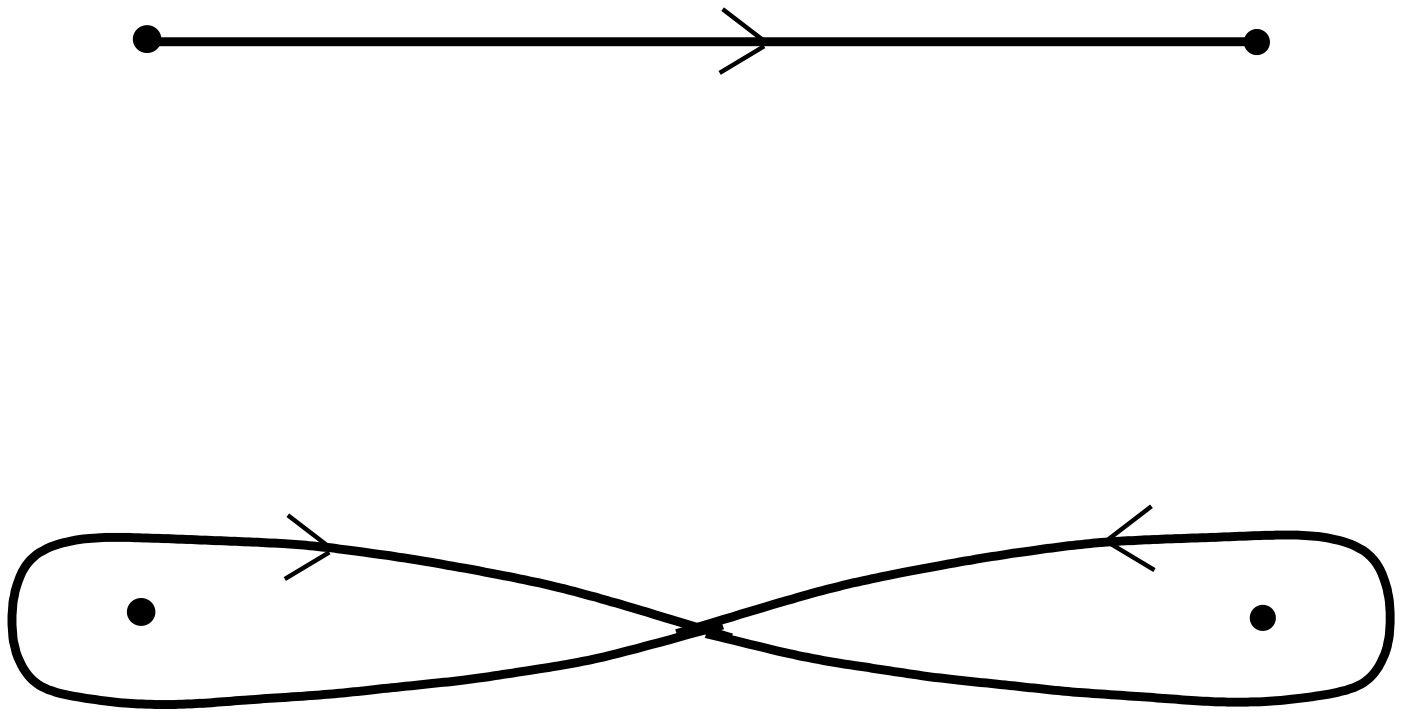
\includegraphics[width=3.5in]{figs/Fig07.png}
 \end{center}
\caption{\small 针 $\CC_{12}$（上）与闭合积分围道（下）的比较，后者等价于 $(1-q^{-1})\CC_{12}$。（原稿第 63 页）}
 \label{compare}
\end{figure}

把针与描述 BPZ 共形块时常用的闭合围道（如图~\ref{compare} 所示）作比较是很有意思的。如图所示，这些围道在同调意义下等价于针乘以一个 $q$ 的 Laurent 多项式。从 Stokes 矩阵的角度看，它们并不像针那样初等。

\subsubsection{有对称性破缺时的单个初级场}\label{onesym}


\begin{figure}
 \begin{center}
     % >>> 原文图 8（原稿第 63 页）
  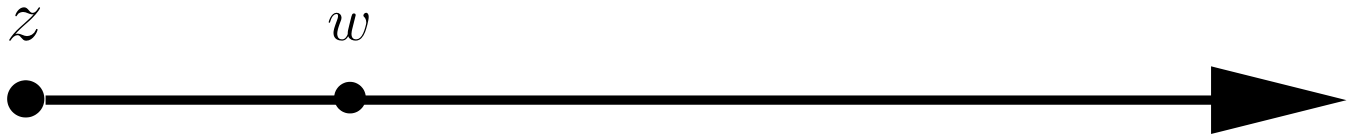
\includegraphics[width=3.5in]{figs/Fig08.png}
 \end{center}
\caption{\small 这条平行于实轴的射线，是存在对称性破缺、且只有一个最小荷初级场时的 Lefschetz 针。（原稿第 63 页）}
 \label{linel}
\end{figure}
另一个只有一个临界点的基本例子出现在存在对称性破缺、并且只有一个 $k=1$ 退化场与一个 Bethe 根的情形。Bethe 方程读作
\begin{equation}
\frac{1}{w - z} =c  \qquad c = - \frac{2 \ca}{\zeta}.
\end{equation}
于是 $w=z + \frac{1}{c}$。为方便起见，我们取常数 $c$ 为实的正数。针再次（图~\ref{linel}）与最自然的积分链 $\CC$ 重合，后者沿一条从 $z$ 出发、平行于正实轴且经过 $w$ 的射线。这个例子说明，存在对称性破缺时，积分链可以终止于无穷远。我们刚刚描述的那条链无法用等价的紧致链替代。

% [Tutor Note: 物理图像] 无对称性破缺时，针的端点只会落在 $w_i\to z_a$（即轻场所在处）；对称性破缺（无穷远处引入非正则奇点）额外提供了 $w\to\infty$ 这一“逃逸出口”，于是同一临界点的针可以终止于无穷远。这正是本小节的要点：紧致围道在同调中不再足以张成整个（扭化）相对同调，必须保留非紧链。

\subsection{两个临界点}\label{twoc}
接下来我们考虑只有一个 Bethe 根 $w$、却有两个临界点的例子。这出现在存在对称性破缺时两个 $k=1$ 初级场的情形，或无对称性破缺时三个此类初级场的情形。

\begin{figure}
 \begin{center}
     % >>> 原文图 9（原稿第 64 页）
  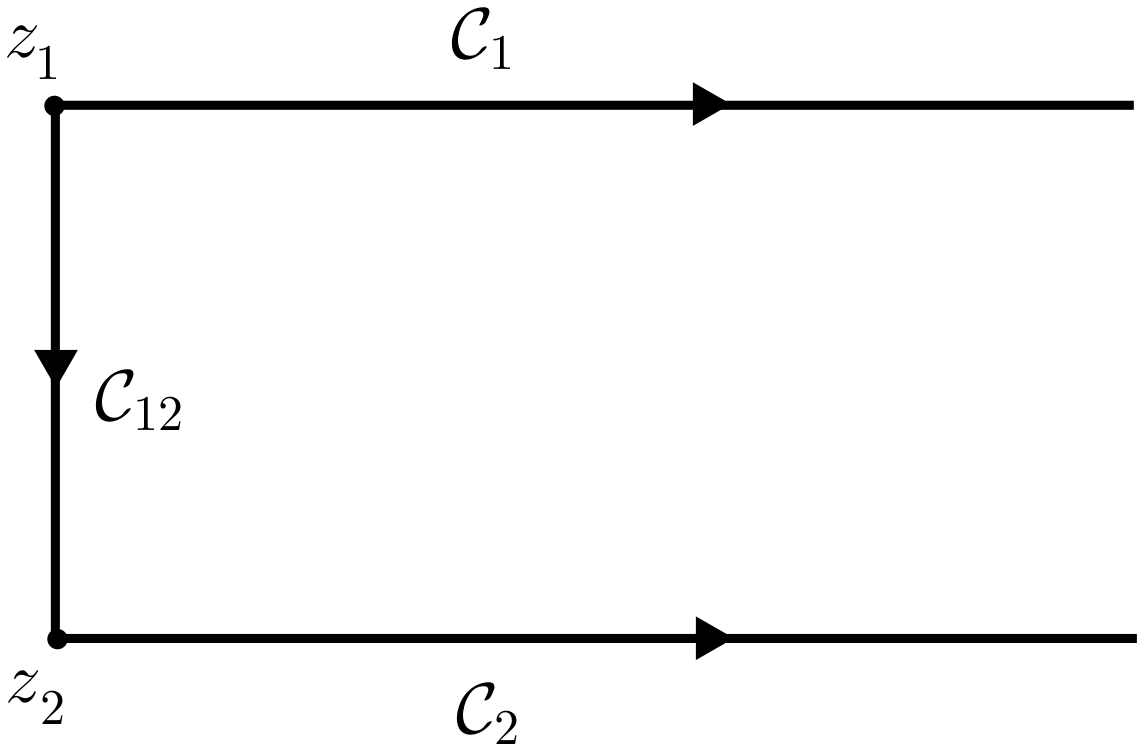
\includegraphics[width=3in]{figs/Fig09.png}
 \end{center}
\caption{\small 链 $\CC_1$、$\CC_2$ 与 $\CC_{12}$。（原稿第 64 页）}
 \label{cyclesonetwo}
\end{figure}
